\documentclass[12pt]{article}

\usepackage[utf8]{inputenc}
\usepackage{latexsym,amsfonts,amssymb,amsthm,amsmath,graphicx}
\usepackage{hyperref}

\setlength{\parindent}{0in}
\setlength{\oddsidemargin}{0in}
\setlength{\textwidth}{6.5in}
\setlength{\textheight}{8.8in}
\setlength{\topmargin}{0in}
\setlength{\headheight}{18pt}

\newcommand{\Lc}{$\mathcal{L}$}


\title{ASTR 206 Lecture Notes}
\author{Simeon Bird}
% \date{October 14, 2019}

\begin{document}

\maketitle

\section{Bayesian Statistics}

``If you need statistics, get a better experiment''

Bayesian statistics is a relatively new branch of statistics which easily allows the combination of multiple information sources and computes a subjective probability of a fact being true, under the currently available information.

Frequentism is concerned with probabilities of events occurring in the long run and works out the probability of some particular dataset occurring under some model. There are then a series of rules for whether this implies that the data is ``true'' or consistent with noise.

Although the two are not technically related, modern Bayesianism relies heavily on numerical computation, while frequentism relies on analytic computations. In practice, analytic usually means Gaussian, as that is the only thing that can be computed easily.

Gaussian approximations are used for two reasons:
\begin{enumerate}
  \item The Central Limit Theorem says everything measured with a large enough sample size is approximately Gaussian (or Normal) distributed
  \item Ease of calculation. Gaussians are easy to integrate.
\end{enumerate}

Bayesian statistics was able to advance because computational power increased. With computers, statisticians can explore distributions that are usually the combinations of different Gaussians, but are not themselves Gaussian, and model experiments in complicated and interesting ways.

\subsection{Bayes' Theorem}
Bayes' Theorem can be written as the following:
\begin{equation}
    P(M|D) = \frac{P(D|M)P(M)}{P(D)}
\end{equation}
In some sense this is just a restatement of the definition of conditional probability:
\begin{equation}
    P(A|B)P(B) = P(B|A)P(A)
\end{equation}
but we are writing down now our amount of belief in a model, not the concrete occurrence of physical events.

\subsection{Notation \& Definitions}
\begin{itemize}
  \item M is a model (an essential part of Bayesianism). You must have a concrete model!
  \item D is experimental data
    \item $P(M|D)$ is the probability of the model given data, the posterior. This is the thing that you want. Note we compute a probability but we have not yet given a decision threshold as to whether the model is true. This is another topic called Bayesian Decision Theory.
    \item $P(D|M)$ is the probability of the data given the model. It is also called the likelihood.
    \item $P(M)$ is the prior: it doesn't depend on data. This is the prior belief in the absence of data. It can model earlier experiments of your own inherent theoretical prejudices. It is in principle subjective and you may validly choose different priors. However, as shown in Figure~\ref{fig:prior_plot}, as long as you choose a prior which is much wider than the posterior, its effect will be mild. If you have a prior that is not wider than the posterior, you need a better experiment!
    \item $P(D)$ is the total probability of the data. This is a strange quantity, naively impossible to compute. Instead we cheat, and find it by using the normalization of probabilities: $\sum_i P(M_i|D)=1$. Note that this asserts that we have considered all possible models, which is never really the case.
\end{itemize}

\subsection{Likelihood}

In some cases, we have a discrete probability of each event, $p^i_f$, and finding overall statistics is a matter of computing binomial probabilities. This is in some ways an ideal case for Bayesian statistics: we wrote down a probability distribution function and then we modelled it. However, even in this case, in practice computation may be difficult for large numbers of events.\\
More commonly, we have continuous parameters in a model. In practice, we often use a multi-D $\chi^2$ or Gaussian likelihood:
\begin{equation}
	\mathcal{L} = P(D|M) = exp(-\sum_{data}\frac{(d_i-m)^2}{\sigma_i^2})
\end{equation}
$d_i$ is datapoint, $\sigma_i$ is error on each point and m is model.\\
If $d_i$ are independent, more generally, the covariance matrix is:
\begin{displaymath}
\mathbf{C} =
\left( \begin{array}{cccc} \sigma_1^2 & \\
& \sigma^2_2 & &\\
& & \ddots & \\
& & & \sigma^2_n
\end{array} \right) \\
\end{displaymath}
A more general likelihood is:
\begin{equation}
	-ln\mathcal{L} = \sum (d_i - m)^T C_{ij}^{-1} (d_j -m)
\end{equation}
where $C_{ij}^{-1}$ is the inverse covariance metrix. It helps if C is diagonal. Generally, people assume that C is independent of m.
There is also a normalisation factor: $\frac{1}{\sqrt{2\pi^n (det C)}}$, which few people compute because the posterior is already normalised.

Note that in practice we often still approximate likelihood functions as Gaussian, but it is important to know that, especially far from the peak, this is rarely a good model. Generally the far tails of a distribution are larger than a Gaussian predicts (see Figure~\ref{fig:gaussian_noise_plot}).

\begin{figure}[ht]
%\includegraphics[scale=0.42]{paper_mf.pdf}
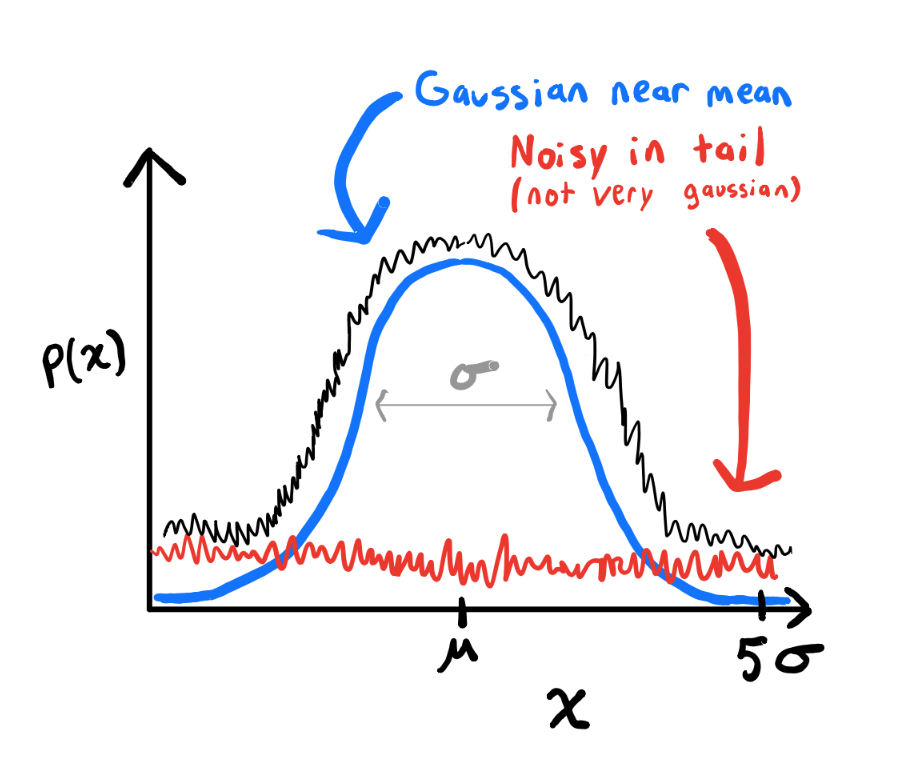
\includegraphics[scale=0.75]{gaussian_noise_plot.png}
\centering
\caption{An cartoon example of most probability distributions in real life. Near the mean (within 1$\sigma$) one can approximate the distribution (black line) as Gaussian (blue line). However, in the tail ($\sim 5\sigma$) the distribution is often fatter (red line).} \label{fig:gaussian_noise_plot}
\end{figure}

Notable examples of people failing to realise this include the 2008 financial crisis and its consequences, as well as forecasts of the 2016 US presidential election.

\subsection{Prior}

In principle, the prior can be anything. However, there are two types of priors that commonly used.

1. We can use the prior to combine old and new experiment.\\
For example, $P(M|D_2) \propto P(D_2|M)P(M)$. $P(M)$ is set using old data. Then $P(M) = P(M|D_1) = P(D_1|M)P(M)$.
For example, we may have an experiment which measures $\frac{G}{R^2}$ and one which measures G. We can use experiment 2 to replace a prior on G in experiment 1 and thus get R. Make sure you use a prior from an experiment which has been done correctly! Using false prior information can lead to bad results.\\
2. Ultimately, we need a starting point, for which we use a minimal information prior. Good choices are a flat, uniform prior: $P(p_i = P_i) = \frac{1}{P_{max} - P_{min}}$. Or a wide Gaussian prior around an order of magnitude estimate.

\begin{figure}[ht]
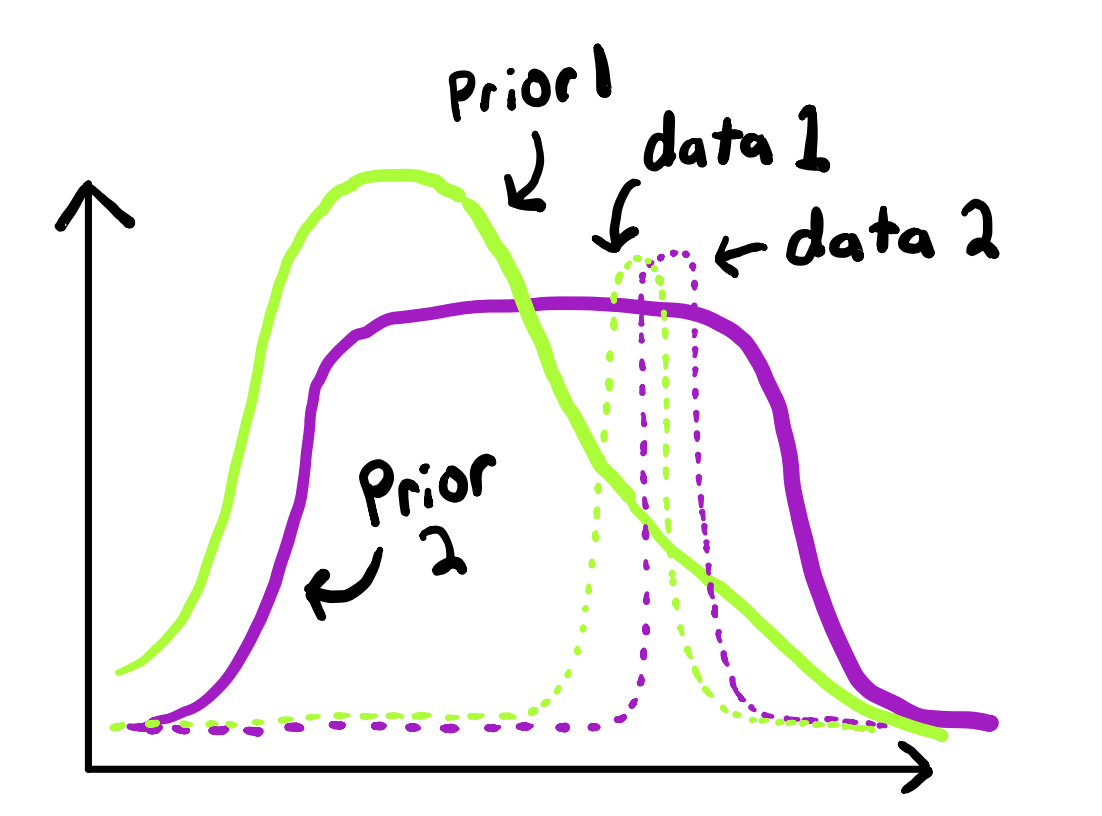
\includegraphics[scale=0.75]{prior_plot.png}
\centering
\caption{An cartoon example of how one's choice of prior can affect the posterior probability (data). Generally, the prior should always be \textbf{broader} than the data.} \label{fig:prior_plot}
\end{figure}

\subsection{Monty Hall}

\noindent There are three cups, and under one cup is a coin.

\begin{figure}[ht]
	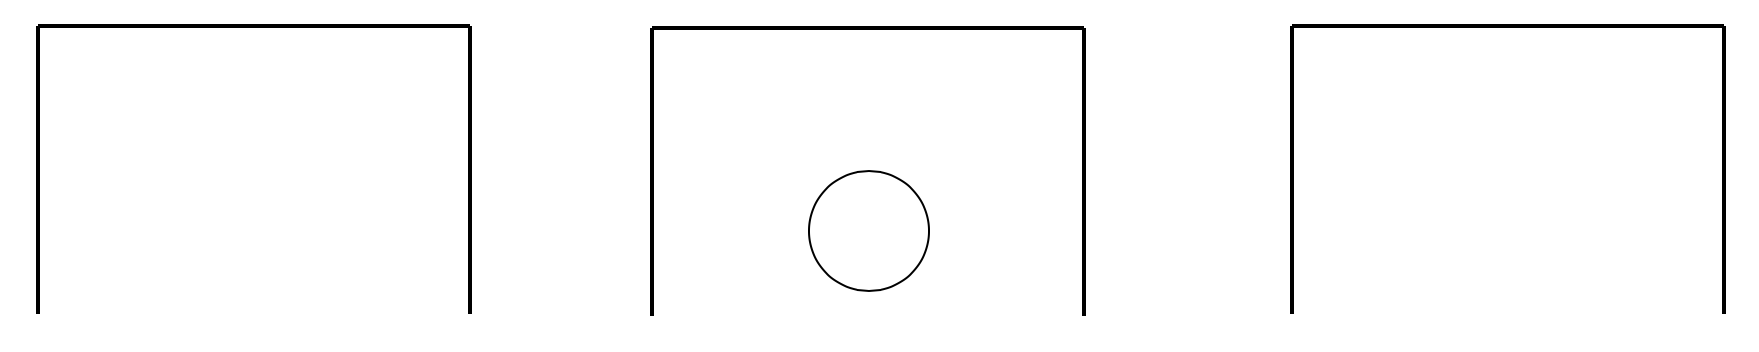
\includegraphics[width=5.0in, keepaspectratio]{Three_Cups.png}
\end{figure}


\noindent You pick one of the cups, and Monty Hall (MH) removes a cup without the coin. What is the probability that your cup has the coin?

\begin{figure}[ht]
	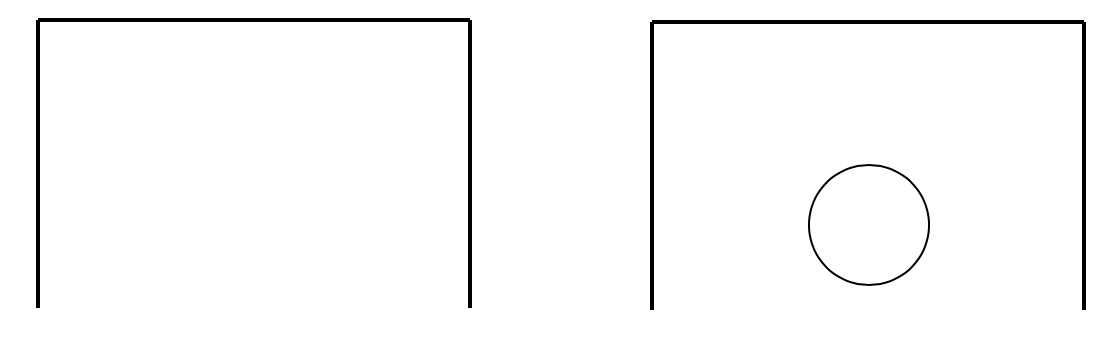
\includegraphics[width=3.2in, keepaspectratio]{Two_Cups.png}
\end{figure}


\noindent Start with P(X=x) = $\frac{1}{3}$, where x = cup 1, cup 2, cup 3. Now consider the scenario that the coin is under cup 1. One way of looking at this is that the probability of your cup having the coin has not changed, so it is still $1/3$ and thus the probability of the other cup having the coin is now $2/3$. Another way is as follows:

\bigskip

\noindent You pick x = cup 1 and it has the coin under it. MH removes cup 2 or 3.

P(X=1) $\cdot$ P(MH removes cup 1) +

P(X=1) $\cdot$ P(MH removes cup 2) + \indent  $\Rightarrow$ \indent  0 + $\frac{1}{3} \cdot \frac{1}{2} + \frac{1}{3} \cdot \frac{1}{2}$ $\Rightarrow \frac{1}{3}$

P(X=1) $\cdot$ P(MH removes cup 3)

\bigskip

\noindent You pick x = cup 2, but the coin is under is under cup 1!

P(X=2) $\cdot$ P(MH removes cup 1) +

P(X=2) $\cdot$ P(MH removes cup 2) + \indent  $\Rightarrow$ \indent 0 + 0 + $\frac{1}{3} \Rightarrow \frac{1}{3}$

P(X=2) $\cdot$ P(MH removes cup 3)

\bigskip

\noindent You pick x = cup 3, but the coin is still under cup 1!

P(X=3) $\cdot$ P(MH removes cup 1) +

P(X=3) $\cdot$ P(MH removes cup 2) + \indent  $\Rightarrow$ \indent  0 + $\frac{1}{3}$ + 0 $\Rightarrow \frac{1}{3}$

P(X=3) $\cdot$ P(MH removes cup 3)


\noindent Regardless of which cup you initially choose, you have a $\frac{1}{3}$ chance of winning, but a $\frac{2}{3}$ chance by switching cups.

This example works (ie, the probability is not $1/2$) because we have prior information about the position of the coin from the initial setup. Even though we did not know where it was, we still were able to learn where it wasn't.

\bigskip


\noindent Books on Bayesian stats

Hogg et al paper \url{https://arxiv.org/abs/1008.4686}

E.T Jaynes - a Bayesian manifesto

C Mackay: Interference - Practical guides to using Bayesian statistics

Gelman: Bayesian Data Analysis - Analysis techniques for various problems.

Ivezic \& others: Orange book: \url{https://www.amazon.com/Statistics-Mining-Machine-Learning-Astronomy/dp/0691151687} - The astrostatistics textbook

\end{document}
